\documentclass[journal,twoside]{JoPhA}
\usepackage[utf8]{inputenc}
\usepackage{flushend}
\usepackage{graphicx}


\begin{document}

\title{VisualHFSM: a tool for programming robots with automata in JdeRobot}
 
\author{Samuel Rey and Jos\'e M. Ca\~nas
\IEEEcompsocitemizethanks{\IEEEcompsocthanksitem Samuel Rey and Jos\'e M. Ca\~nas are with Universidad Rey Juan Carlos\protect\\

E-mail: s.reye@alumnos.urjc.es, josemaria.plaza@urjc.es
%\IEEEcompsocthanksitem Vicente Matell\'an is with University of Rey Juan Carlos.
} % <-this % s
}

\markboth{Journal of Physical Agents,~Vol.~1, No.~1, July~2007}%
{Cazorla and Matellan : JoPhA Paper Demo}
\maketitle


\begin{abstract}
A visual programming tool, named VisualHFSM, has been improved in the JdeRobot robotics software framework. This tool provides Hierarchical Finite State Machines to program robot behaviors. The particular automata is designed visually, with nodes for the states, links for the transitions and specific source code on them. It automatically generates a C++ or a Python JdeRobot component that connects to the drivers and implements the automata. It uses multithreaded templates for that. Such component dynamically shows the current state of the automata while it is running. This tool speeds up the development time of robot behaviors, reducing the code that has to be created from scratch for new behaviors. VisualHFSM has been experimentally validated creating several autonomous behaviors for drones.
\end{abstract}


\begin{IEEEkeywords}
Visual languages, robot programming, automata
\end{IEEEkeywords}


\section{Introduction}

\IEEEPARstart{M}ost of the robot intelligence lies on its software. Its functionality resides in its programming, in the software that manages hardware resources like sensors and actuators. There is no universally standardized methodology to program robots. In the last few years the robotics community has begun to apply software engineering methodologies to its field, making more emphasis in code reuse, distributed software design, etc. Several robot programming frameworks that simplify the development of applications have emerged. 

These frameworks (1) provide a more or less portable hardware access layer (HAL); (2) offer a concrete software architecture to the applications; (3) include tools and libraries with already ready-to-use functionality and building blocks. Many of the emerged platforms are component oriented, such as ROS, Orca, Microsoft Robotics Studio, RoboComp, JdeRobot, etc..

Another interesting tool that can be used for robotic software development is the use of automatons to generate robot behaviors. Finite State Machines (FSM) have been succesfully used to symbolize the robot behaviors, representing them in a compact and abstract form. With FSM the behavior is defined by a set of states, each of which performs a particular task. The system can then switch from one state to another through transitions, which are conditions of state change or stay depending on certain events or sensor conditions that may happen, both internal or external. FSMs provide one smart way to organize the control code and perception on-board a mobile robot. They have been explored in research and also incorporated in recent robotic frameworks with tools that let the programmer to focus on the behavior logic more than in implementation details. With these tools most of the code is then generated automatically from the abstract description of the FSM. This diminishes the chance of bugs, reduces the development time and allows the programming of complex behaviors in a robust way.

%paper goal
JdeRobot is the component oriented robot programming framework developed in Universidad Rey Juan Carlos. In this paper we present the new release of the VisualHFSM tool in JdeRobot, which supports the visual programming of robot behavior using hierarchical Finite State Machines. Now it can generate Python components, not only C++ ones. The generated components now show their dynamic state (the active states in the hierarchical FSM) while running. And its usability has been improved.

%paper organization
The reminder of this paper is organized as follows. In the second section we review related works on FSM tools in different frameworks. The third section presents in detail the current visual programming tool, VisualHFSM, noting the improvements from the previous release. The fourth section describes two example applications generated with VisualHFSM, two robot behaviors of a simulated drone. Finally, conclusions are summarized.

\section{Related works}
%Smach
Regarding  finite  state  machines,  ROS  is  also  gaining prestige with its platform-independent SMACH \footnote{http://www.ros.org/wiki/smach} \cite{boren2010,bohren2011}. This tool is a task-level architecture for rapidly creating complex robot behaviors. At its core, SMACH is a ROS-independent Python library to build hierarchical finite state machines. To develop a hierarchical finite state machine you have to write the code needed to create and describe each state and transition, it is not a visual tool. The package also comes with the SMACH-viewer %(Figure \ref{fig:smach})
, a tool that shows the developed finite state machine at runtime. In that tool, we can see either a graph or a tree view of the current automaton, but not both at the same time. It also shows every state and transition, as well as the active state and a debug window where we can see data of the active state.

%\begin{figure}[ht!]
%\begin{center}
%        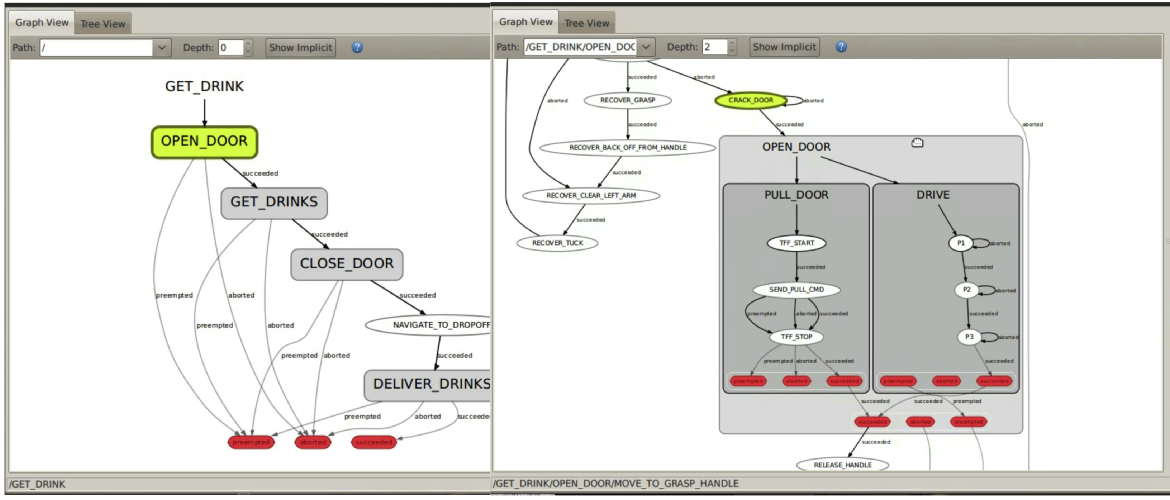
\includegraphics[width=8.5cm]{figs/smach-viewer.png}
%\end{center}
%\caption{An instance of SMACH-viewer}
%\label{fig:smach}
%\end{figure}

%MissionLab
One of the most powerful frameworks that use HFSM in robotics is MissionLab, developed in Georgia Tech by the professor R. Arkin. This environment includes a graphical editor of  configurations  (CfgEdit) \cite{mackenzie1998} as a tool, similar to  automaton,  that  allows  to  specify  missions  with  its states, transitions, etcetera. It allows to generate applications following the AuRA architecture, developed by the same group. In order to represent the automaton they developed their own language, the Configuration Description Language. A more recent example of FSM is the automaton editor inside the component-oriented platform RoboComp, from Universidad de Extremadura. For instance, in \cite{cintas2011}, they used it to program the behavior of a forklift. Another sample is the behaviors graphical editor Gostai Studio \cite{gostai2012}, inside the Urbi platform. This graphical editor generates urbiscript code as its output, includes time-execution visualization of the state of the automaton, allows to stop and continue the execution of the generated automaton and offers the possibility of creating hierarchical finite state machines.

%XABSL
In the RoboCup scenario finite state machines are frequently used to generate behaviors for the standard SPL league humanoid robots. Several teams use the tool and language XABSL \cite{lotzsch2004,risler2009} to specify behaviors, around the influential German team B-Human. In addition, the TeamChaos team \cite{herrero2006} used an HFSM tool to handle hierarchical finite state machines for its architecture ThinkingCap, allowing even behavior hot-edition in each state. In the SPIteam team a tool named Vicode is used to generate finite state machines for BICA architecture.

Another  example  of  the  automaton  power  is  the  use for programming the intelligence of automatic players in videogames. This scenario is simpler than real robotic because much of the player perception is obtained looking up some videogame variable. For instance, in the successful Halo 2 of Bungie automaton trees were used to deploy more than one hundred different behaviors.

%Xait, videojuegos 
Xait \footnote{http://www.xaitment.com} enterprise  commercializes  tools  that  facilitates automaton programming to videogames developers, as its xaitControl %(Figure \ref{fig:xaitcontrol})
. This tool allows the programmer to  easily  develop  behaviors  with  hierarchical  finite  state machines. It has a main canvas in which the automaton is displayed, a tree view on the left shows the created structure and other panels show different information about auxiliary procedures, execution flow control, etc.

%\begin{figure}[ht!]
%\begin{center}
%        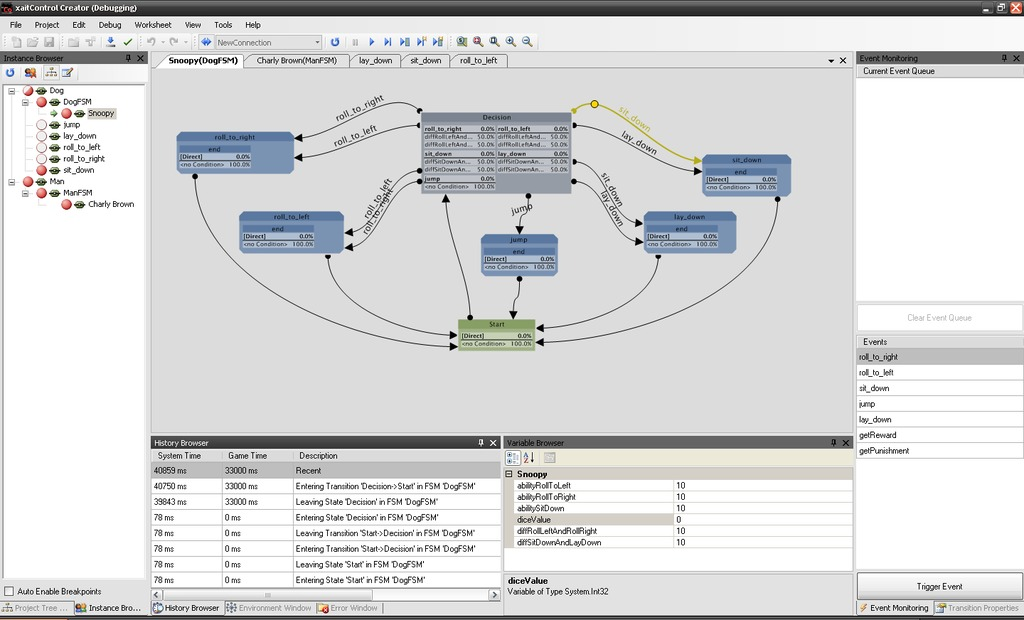
\includegraphics[width=8.5cm]{figs/xaitcontrol.jpg}
%\end{center}
%\caption{An instance of xaitControl}
%\label{fig:xaitcontrol}
%\end{figure}

%refs de Joaquín y sus redes de Petri


\section{VisualHFSM}
%general presentation
VisualHFSM is a tool created for the programming of robot behaviors using hierarchical finite states machines (HFSM – Hierarchical Finite State Machines). It generates as output a component in JdeRobot framework that implements the robot behavior. Even if it is not a visual programming language itself, it is inspired on them, as VisualHFSM represents the robot’s behaviour graphically on a canvas composed of states and transitions. 

The source code to be executed in each state or transition can be introduced. This tool decreases the development time for new applications, providing the developer with a higher level of abstraction. It also increases the quality of these applications, automatically generating most of the code using a clean and well organized template, so the tool allows the engineer to focus on specific parts of his application, writing only the actual code that will be executed by the automata and the conditions that will make the robot go from one state to another. As a consequence, the final result is a more robust code and less prone to failure. 

% explained before, VisualHFSM is a flexible tool that allows its users programming code for several different type of robots, saving time by focusing only in programming the code that actually depends on the automata behaviour, and auto-generating the complete code of the automata by completing a template, achieving in this way a robust and well organized code minimizing the effort of the developer.


%visualHFSM parts
VisualHFSM is divided in two parts: a graphical editor and the automatic code generator. The graphical editor displays the main window of the tool, where all functionality is located to create the automata structure. It also contains internal structures that provide functionality to the interface and saves all the data related to this automaton in an XML file. %The aspect of this graphical editor in VisualHFSM is shown in the figure \ref{fig:editor}. 

The automatic code generator reads the XML file that was created and saved using the graphical editor, and delivers the source code of a JdeRobot component implementing the HFSM. It also generates a .cfg file created from the parameters passed through the graphical interface and a CMake file for compiling the automata. The compiling is also done using the main window of the graphical editor, and it will leave an executable file in the path where the XML has been saved.

%It has a graphical editor and an automatic code generator. The graphical editor still displays the main window where all functionality is located to create the automata, and all of this functionality that compose the automata is saved inside a XML file. The main changes are related to the automatic code generator, as explained before, it generates C++ and python code.  This will be explained in more detailed in the following sub chapters. 

\subsection{Graphical editor}

The graphical editor allows the user to visually represent, edit and add states and transitions in a clear and simple way. The component is represented by a finite state machine in a canvas, where all elements are visualized. It allows to manipulate states (create, remove, move, rename...) and to define the behavior that will be executed in them. It is also possible to set the conditions for regulating the transitions between states, and the code that will be executed when the transitions occur.

\begin{figure}[ht!]
\begin{center}
        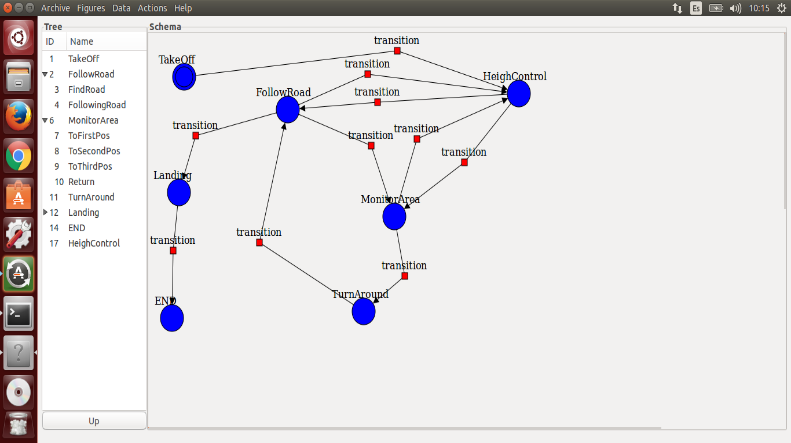
\includegraphics[width=8.5cm]{figs/editor.png}
\end{center}
\caption{Graphical editor of VisualHFSM 5.0}
\label{fig:editor}
\end{figure}

As shown in the Figure \ref{fig:editor}, the GUI in VisualHFSM 5.0 is now divided into two parts (instead of three of previous releases, like that on Figure \ref{fig:editor-old}): the \texttt{Tree View} at the left and the \texttt{Scheme View} at the right. The third part presented in previous releases is now placed in the \texttt{menu bar} on the top and has more functionalities. By doing this, the space of the window for creating the automata’s scheme is bigger, so it is more comfortable draw on it. Also, the canvas, the \texttt{Tree View} and all of the popup elements are scrollable.

\begin{figure}[ht!]
\begin{center}
        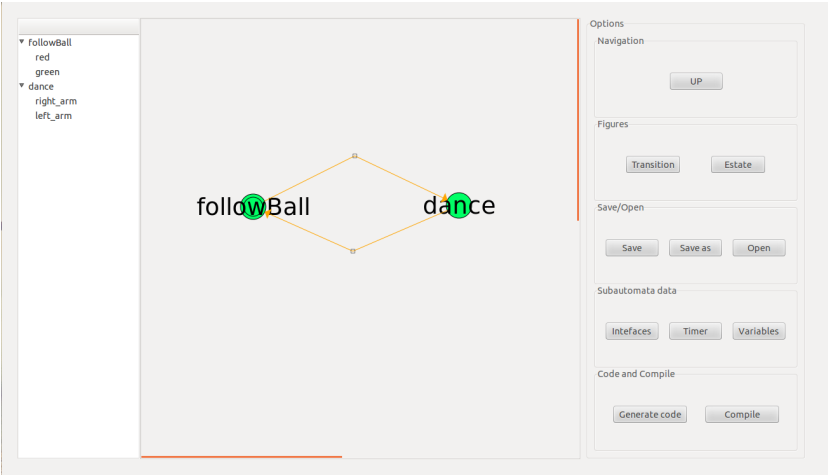
\includegraphics[width=8.5cm]{figs/editor-old.png}
\end{center}
\caption{Graphical editor of previous version of VisualHFSM}
\label{fig:editor-old}
\end{figure}

The \texttt{Tree View} is the area placed at the left of the window, where all the automata is text represented in the hierarchical mode with two columns for identifying the states: one for the ID and other for the name given to this state. It has the option of collapsing or expanding the children of some state, so the developer can choose to see all the levels at the same time or focus on some specific levels by collapsing the rest. The children and levels of the hierarchy are represented under their fathers by using different tabulations. The Tree View allows a simple and intuitive navigation through the automata, as it allows to make double click in one state for representing the subautomata that contains it in the Schema View.

The \texttt{Schema View} is a canvas where the automata is drawn, showing the name of each element, either state or transition. States are represented as blue circles and for each subautomata it also marks with a double circle the state which must be active at the beginning. For each state, the user can rename it; edit it, allowing to change the code of the selected state; mark it as the initial state of its subautomata; copy it, allowing to paste the selected state into another or the same subautomata; and delete it. Any state can be connected to another by an unlimited number of transitions or to itself by auto-transitions. Transitions are represented as arrows that go from the origin state to the destiny, with a red square in the middle for applying them different actions, as move them, rename them, editing its condition, adding them code and delete them. The condition added by editing a transition is the condition that must happen for the transition to happen. The Schema View also allows to graphically navigate through the automata. For going to the child subautomata of any state is enough with doing double click in the desired state. For going back to the upper level, there is the “Up” button, just under the \texttt{Tree View}.

In the \texttt{menu bar}, menus are structured in five groups: Archive, Figures, Data, Actions and Help. The Archive menu allow to create new projects, open existing ones, saving the current project or exit VisualHFSM. Figures menu contain two buttons, for adding new states or transitions. Data menu has Timer, for choosing the frequency of the iterations, and Variables, for adding variables and functions that the developer may need for better organizing and structuring its code, giving more flexibility to the tool. Lastly, the Actions menu allows to add additional libraries that the automata code may need, edit the parameters for the “Config file” that will be auto-generated with the code, generate C++ or python code and compile the C++ code by using the CMake file generated with the code.

\subsection{Automatic generation of C++ component and its runtime GUI}

For running the automata (with the states, transitions, and other data specified through the editor), the XML file is parsed and a new JdeRobot component in C++ is generated. Such C++ component implements the automata and is generated using a carefully designed \textit{C++ template}. Each subautomata is implemented as a single thread, so the full automata is a collection of concurrent threads which interact among them, sleep, are resumed, etc. as some states of the automata are activated or deactivated. More details of this template can be found in \cite{borja2013}.

In the new VisualHFSM 5.0 some code to graphically show the (hierarchical) automata state at runtime has been included. If the user wants it, the generated JdeRobot component may display an additional runtime GUI that shows which states are active or not while running. This is powerful debugging functionality. The developer may check in a natural way whether the robot’s behavior is the same as expected, or whether the automata transits from one state to the intended one.

\begin{figure}[ht!]
\begin{center}
        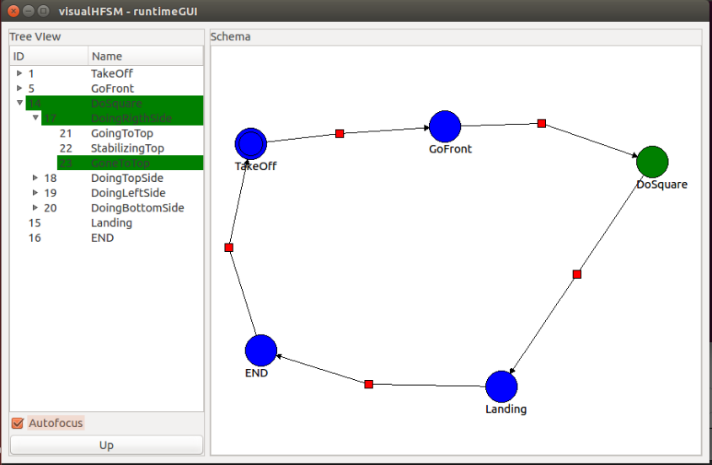
\includegraphics[width=8.5cm]{figs/runtime.png}
\end{center}
\caption{Runtime GUI in C++ component using the Autofocus feature}
\label{fig:runtime}
\end{figure}

%use
Figure \ref{fig:runtime} shows one runtime GUI, which looks like the graphical editor window. It also has two sections, the Tree View and the Schema View, but instead of allowing editing the automata, it represents the states that the automata is currently executing. 

For indicating which states are active, the Tree View colors the background of the current active state as green. This includes the root state and all its active children, so it the active states in all levels of the hierarchy. As in the graphical editor, the user may expand or collapse the different hierarchical levels at will. The grahical navigation inside the automata works as in the graphical editor. In addition, under the Tree View is a check box named “Autofocus”. When activating this, the Tree View will automatically expand and collapse itself for showing the active states expanded and the rest of the automata will be collapsed, for allowing an easier perception of the actives states, as shown in Figure \ref{fig:runtime}. In the Schema View of this runtime GUI, the active nodes are presented in green and the others in blue, and again, the navigation works as in the graphical editor. When a transition takes place, the old active state is painted in blue in the Schema View and in white in the Tree View, and the new active state is painted in green. 

This runtime GUI feature is off by default, because the graphical window is useful only for debugging. In normal robot operation, once its behavior programming has been refined, there is need to spend computational resources in this additional GUI. Nevertheless, it is very useful in the developing process. Enabling this feature is as easy as executing the component with the flag \texttt{--displaygui=true}. If the component is executed by default, the runtime GUI will not be created, so it will have no impact in the robot’s performance.

%implementation
The runtime GUI has been implemented as an additional thread and a new library called \texttt{automatagui}. This library includes all the functionality for using the runtime GUI. %At run time the component does not require the XML file created by the graphical editor. 
When the code or the C++ component is being generated, with the XML already read, a C++ function is written for constructing a list containing all subautomatas with its states and transitions. An object of the class \texttt{AutomataGui} is created and inserted in the generated component. The component will use at runtime the data of that function for graphically showing the automata. That object will also be responsible for changing the color of the states when the active state changes. To avoid race conditions on doing so, when a state is going to be active the thread responsible of executing this subautomata code sends a notification to the GUI thread using a Dispatcher object, and the \texttt{AutomataGui} object will do the rest. 

\subsection{Automatic generation of Python component and its runtime GUI}

In the new release of VisualHFSM, the robot behavior (for the states or the transisitons) may be programmed in Python too. Adding support for this language, VisualHFSM increases its flexibility, which is one of its stronger features. Not only several real robots as Pioneer from ActivMedia, Nao from Aldebaran, ArDrone from Parrot or simulated robots in Gazebo are supported, it also accepts different languages, C++ and python, to program them. 

The only difference while using the graphical editor of VisualHFSM to generate Python components is that the code inserted in the states and transitions must obviously be in Python, but for the rest it works exactly in the same way as when generating C++ components. 

The main difference starts when generating the code, as the template is different. The code is now organized following an object oriented model. There will be the main class \texttt{Automata}, which will contain all the information related to the automata. This approach makes easier the communication between different subautomatas, or different threads, by using elements of the \texttt{Automata} class instead of global variables. It also provides a threading lock, in case some code is sensitive to race conditions and it allows to create inner classes, in addition to more functions or variables that could be needed. The additional features will also be created inside the \texttt{Automata} class. This implementation provides more robust and even better organized and cleaner code. In addition, as Python do not need to compile, it is faster to make any change on the program. The Python code will be generated as an executable, so it can be called in the same way as the C++ executable.

Regarding the runtime GUI, it works in the same way as with C++, the component must be launched with the \texttt{--displaygui=true} parameter for using the runtime GUI feature. The main difference is that it uses a newer graphic library, PyQt4. Also, the way of communicating that the color of a state needs to change is simpler. It is implemented by the GUI thread again to avoid race conditions, but this time the notification is done using a handler. The thread that is going to change its active node will emit a signal with the node name, which will be handled by a handler in the GUI thread. After the notification, the processing is the same as it was in the C++ component. 

In this release it is possible to create several runtime GUI windows (one for one subautomata in detail), in case it is convenient. For unfolding those windows, it is only necessary to do right click over one state of the desired subautomata and then select “Open Subautomata”. This is shown in the Figure \ref{fig:runtime-hierarchy}.

\begin{figure}[ht!]
\begin{center}
        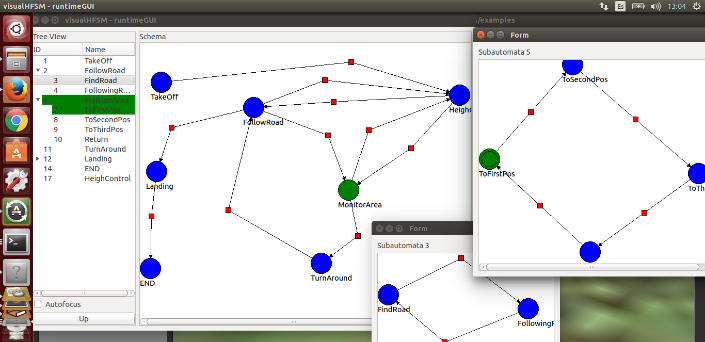
\includegraphics[width=8.5cm]{figs/runtime-hierarchy.png}
\end{center}
\caption{State diagram of the monitor-an-area application shows three subautomatas at the same time}
\label{fig:runtime-hierarchy}
\end{figure}

Another feature added in this release, both in Python and in C++, is the \texttt{Shutdown} function. This function ends the loop of all the subautomatas by setting the correspondent variables to false, so the code will reach the end and finish, in contrast with previous releases of VisualHFSM, where the execution never ended unless the process was manually interrupted from the terminal.

\section{Experiments}

In order to validate the new features introduced with this version of VisualHFSM, we have performed two different experiments, both of them using a simulated ArDrone robot (examples with previous releases of this tool were performed with the Pioneer robot and the Nao humanoid). The experiments are the developments of two robot applications using visualHFSM: monitor-an-area application and follow-colored-objects applications. Both of them are written using the Python code generator of VisualHFSM.


\subsection{Monitor-an-Area application}
%application description
For this first application, we have used a Gazebo scenario with a road, and some victims of a car accident laying in the ground around the location were the accident has occured. This simulated scenario is a example of an application where drones could be useful: go fast to the accident place and check with its camera the status of the victims, for the emergency service to give a better, faster and more accurate response. 

%HFSM-based solution
We identified several states to unfold different behaviors of the robot in this example. Their combination into a HFSM fulfils the whole application. First, the drone has to take off. When it has reached the desired height, it goes to the next state \texttt{following-the-road}. Figure \ref{fig:followingRoad} shows the ArDrone following the road in that state. This state has a child subautomata, for following it and consider other aspects at the same time. For instance, if the drone lost the road, this child subautomata took control to search and recover the road again. After finding it, it returns to the state of following it. 

\begin{figure}[ht!]
\begin{center}
        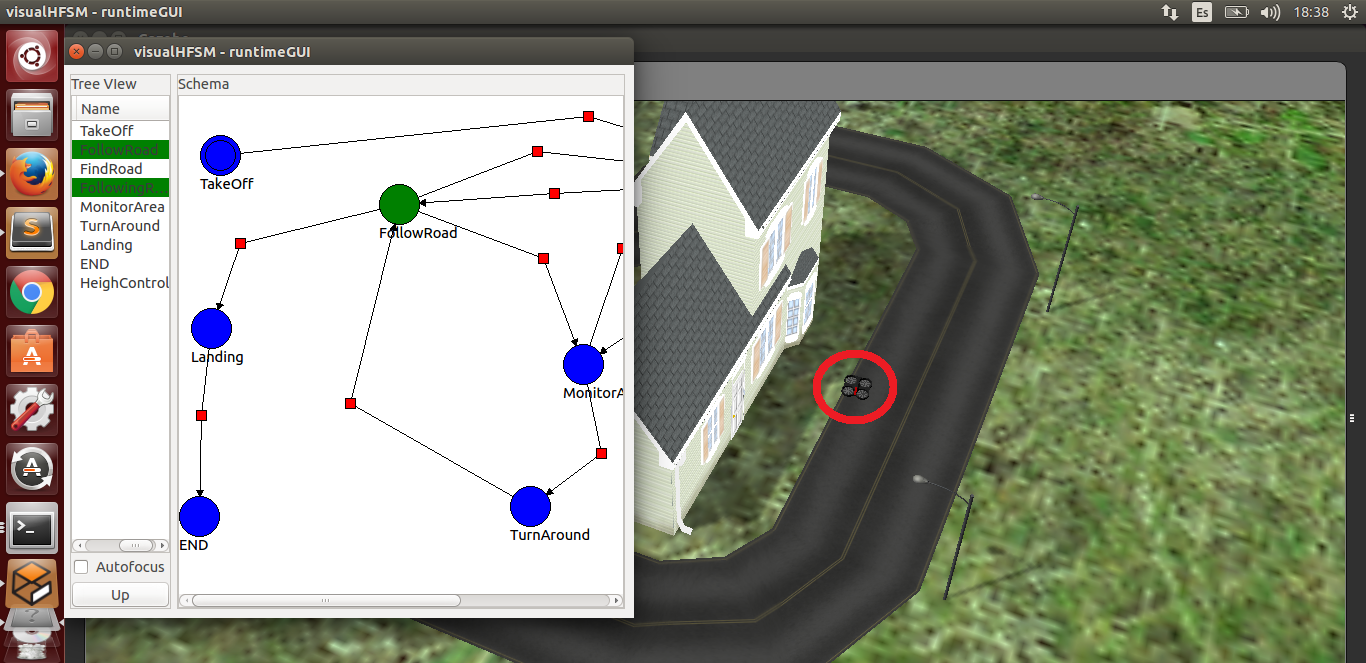
\includegraphics[width=8.5cm]{figs/followingRoad.png}
\end{center}
\caption{ArDrone following the road}
\label{fig:followingRoad}
\end{figure}

It will keep in the \texttt{following-the-road} state until it gets to the point where the accident has happened. Then, it switches to the \texttt{monitor-area} state, which is responsible of looking for and locate the victims, as shown in Figure \ref{fig:watchPerson}, where the drone has found a victim. Once again, this state has a child subautomata for specifying phases of this activity in a simpler and more understandable way. 
When it has finished searching in the area, the drone will come back to the point of the road where it started to search for victims, it will turn around, and again it will go to the \texttt{following-the-road} state, following it until it reaches the point where the drone took off, and then lands there. 

During all the execution, the height of the drone has been watched. If it went too hight or too low, the automata would have switched to another state until it reaches the desired height. The state diagram of this behaviour is shown in the Figure \ref{fig:runtime-hierarchy}, where we can see the root subautomata, and those of \texttt{following-the-road} and  \texttt{monitor-area} states. 

\begin{figure}[ht!]
\begin{center}
        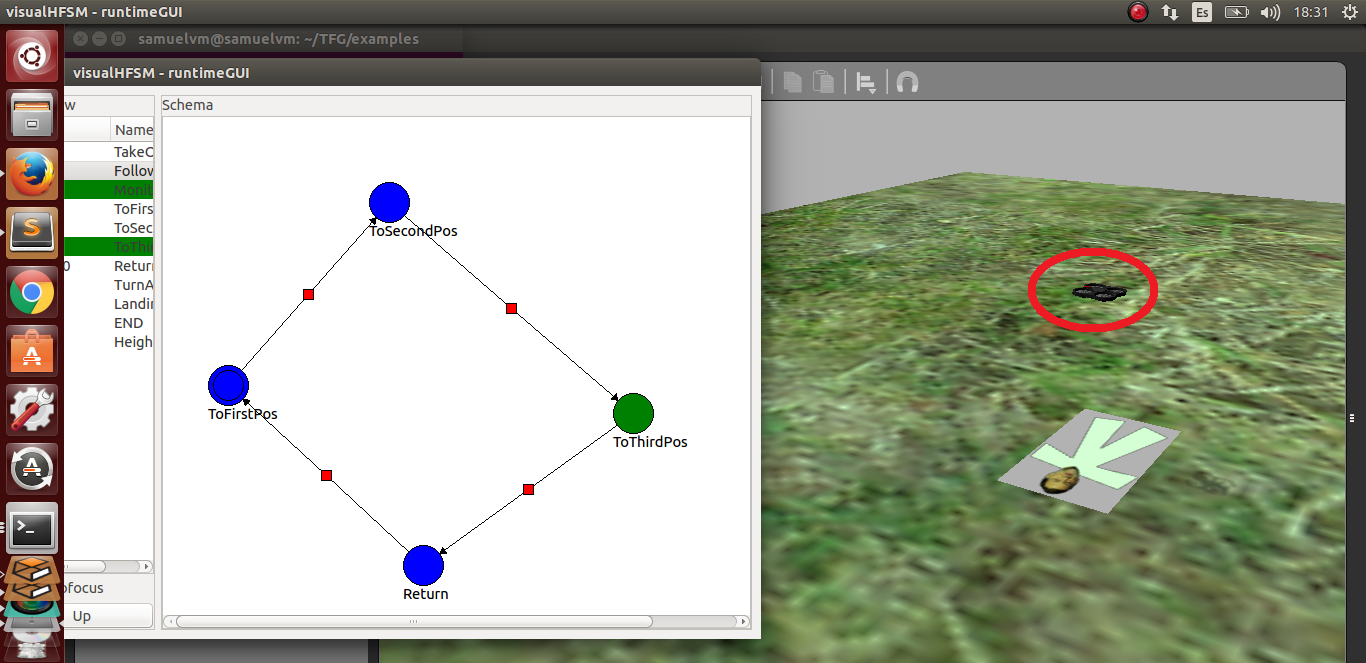
\includegraphics[width=8.5cm]{figs/watchPerson.png}
\end{center}
\caption{ArDrone recording the location of a car accident's victim with its camera}
\label{fig:watchPerson} 
\end{figure}

\subsection{Follow-colored-objects application}
%application description
In this application there are several mobile colored objects in the scenario and the drone has to follow them using its ventral camera under certain circumstances. The sequence that the drone has to follow is green object, then a blue one, then a green one again and finally a red one. This type of behaviour can perfectly be represented using a hierarchy finite state machine, and can not be implemented with a pure reactive behavior.

The sequence starts with the drone looking and following a green object. In this state it will ignore the red objects, but if it sees the green object, the drone will start following it. It will be tracking it until a blue object appears. Then it will follow the blue object for a while, after a new green object appears. In such a case, it will stop following the blue and start following the green again, but now, the blue object will be ignored. While following this green object, it will be also looking for a red object. Once the red has been found, it will starts following it for a while until the program ends. 

\begin{figure}[ht!]
\begin{center}
        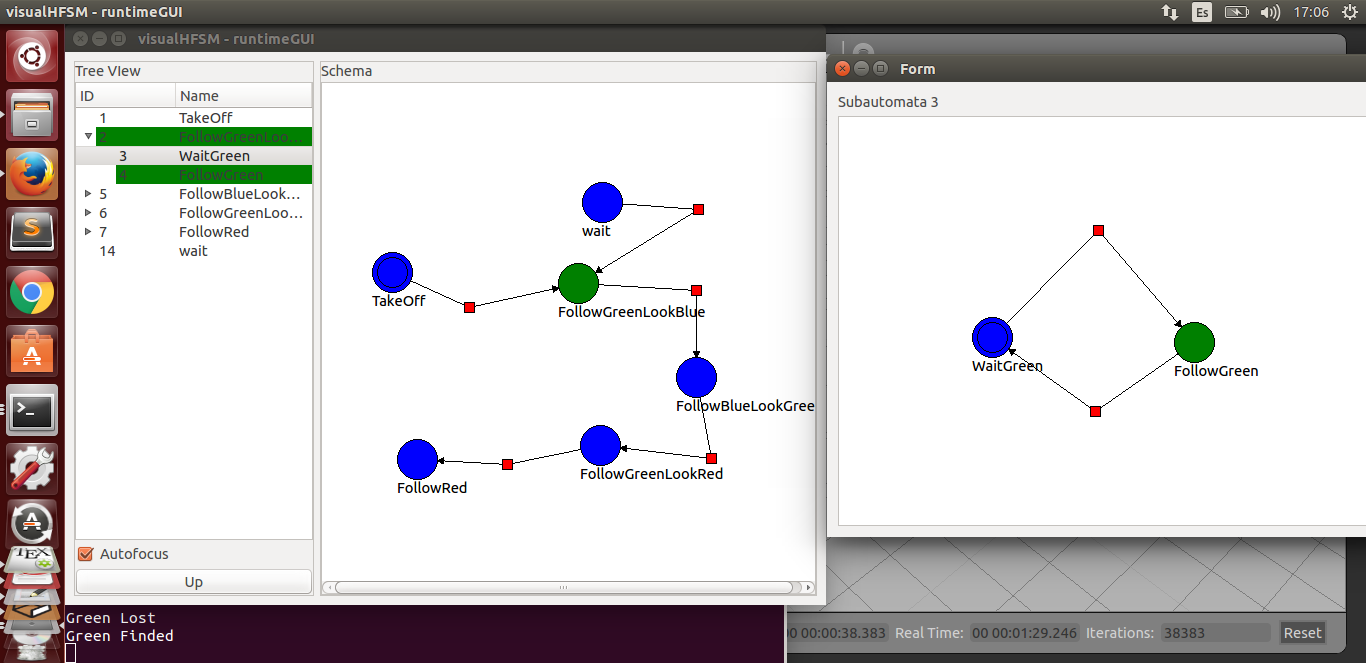
\includegraphics[width=8.5cm]{figs/statesDiagramColors.png}
\end{center}
\caption{State diagram of the follow-colored-objects application from its runtime GUI}
\label{fig:statesColors}
\end{figure}

%implementation
For programming this behaviour, the state diagram in Figure \ref{fig:statesColors} has been used. As it shown, the drone starts with the \texttt{take-off} state. When the desired height is reached, the drone will go to the state \texttt{FollowGreen-LookForBlue}, where it will be filtering two colours: green and blue. It will be following the green object until it detects a blue contour, and then it will pass to \texttt{FollowBlue-LookForGreen} state. This time, to avoid the drone immediately detecting the green object it has been following in the previous state, it will wait a blanking time. During this time it will only follow the blue without looking for the green color, but after it the drone will also look for the green color, passing to \texttt{FollowGreen-LookForRed} state once the drones finds a green object. This state works like the other two, and when the drone finds the red colour it will pass to \texttt{FollowRed} state until the program finishes. 

All the color following states are implemented with a child subautomata. The father looks the color and makes the decision of continuing in this state or transit to another, and the child subautomata performs the tracking. In case the drone cannot detect any of the specific colors, it will stay still. An example of one child subautomata is shown in Figure \ref{fig:statesColors}.

This experiment has already be successfully performed using Gazebo simulator, where the colors are represented by three pioneer robots with their chassis painted on green, blue and red. Figure \ref{fig:followGreen} shows the drone following the green Pioneer while it is ignoring the red one because it is looking for the blue Pioneer.

\begin{figure}[ht!]
\begin{center}
        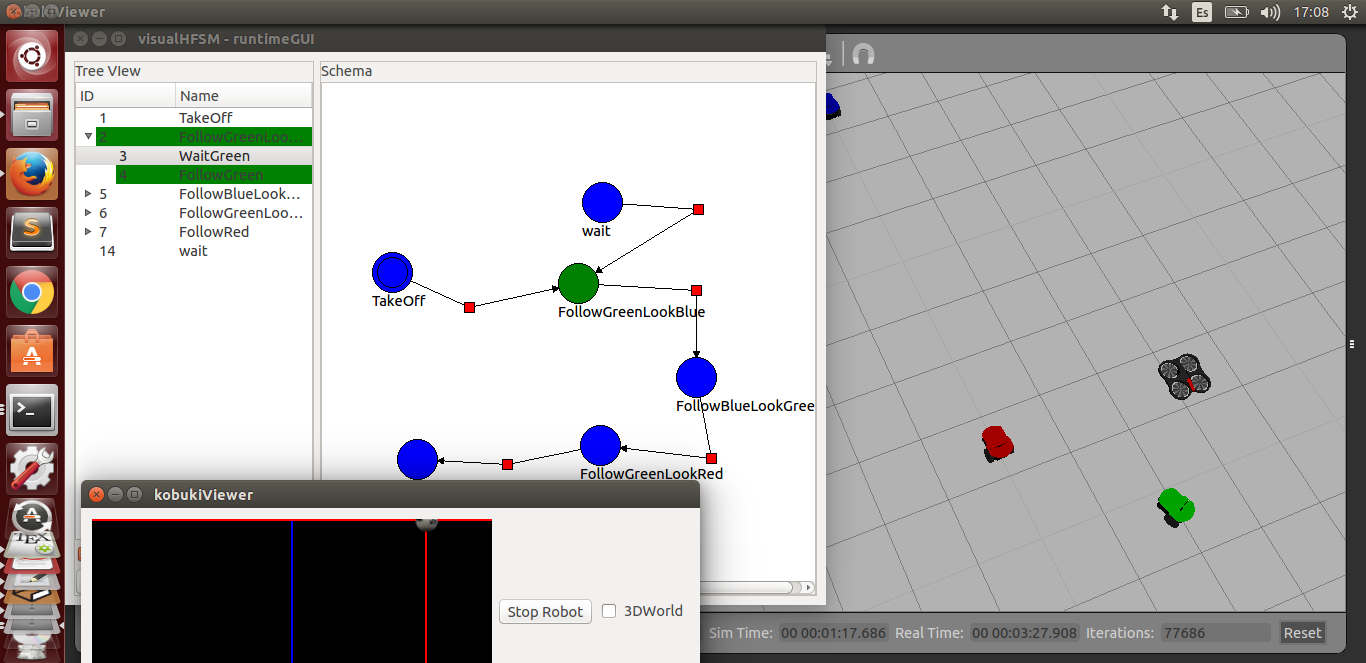
\includegraphics[width=8.5cm]{figs/droneFollowingGreen.png}
\end{center}
\caption{ArDrone robot following a green Pioneer in the Gazebo simulator}
\label{fig:followGreen}

\end{figure}


\section{Conclusions}

This paper has presented the visualHFSM tool in JdeRobot framework. It allows the programming of robot behaviors using automata. The developer creates a graphical representation of the automata, fills the code to be executed on each state and on each transition, and the tool automatically generates the output JdeRobot component. The use of \textit{hierarchical} automata provides power to the tool to represent complex behaviors. The new release automatically generates Python or C++ components, and the generated component dynamically shows the state of the (hierarchical) automata in execution while running. In addition the usability of the tool has been improved.

%The main objective of this version of VisualHFSM is to convert it into a tool that will actually be used for people, and not only for its developers. For doing so, we have improved the flexibility of the tool by adding it an automatic code generator of python, so now it supports both languages: python and C++. Also, a feature that was lost when the hierarchy was introduced, as it was not compatible at first, has been recovered. This feature is a runtime GUI that helps with the debugging process by showing the states and transitions of the automata and its activity. In addition, a more complete and detailed documentation has been created, inside the JdeRobot web page, with detailed examples for allowing new users an easier first contact and understanding of this tool and how it works.

The tool was previously tested with Pioneer and humanoid robots. The new release has also been validated generating two example behaviors for a drone robot. 

%future lines
%We are working in the real case, because the drone is not as stable as they are in the simulator, and good colour filters using real lights are harder to get, but we expect to have images and a video of this soon (before the article publication).
As future lines we would like to promote the use of visualHFSM among JdeRobot users, to get feedback from them using the tool in different scenarios. In this way, the tool has recently been included in the official release of the framework. In addition, we are exploring the extension of the tool to support the Petri nets as robot behavior model.

\section*{Acknowledgment}
This  research  has  been  partially  sponsored  by  the Community of Madrid through the RoboCity2030-III project (S2013/MIT-2748), by the Spanish Ministerio de Economía y Competitividad through the SIRMAVED project (DPI2013-40534-R) and by the URJC-BancoSantander.
%CVIP.

\begin{thebibliography}{1}

% \bibitem{IEEEhowto:kopka}
% H.~Kopka and P.~W. Daly, \emph{A Guide to \LaTeX}, 3rd~ed.\hskip 1em plus
%   0.5em minus 0.4em\relax Harlow, England: Addison-Wesley, 1999.

\bibitem{borja2013}
Borja Men\'endez and Rubén Salamanqu\'es and Jos\'e M. Ca\~nas, \emph{Programming of a Nao humanoid in Gazebo using Hierarchical FSM}.  Proceedings of XIV Workshop on Physical Agents, WAF-2013, pp 15-22. ISBN: 978-84-695-8319-7. 2013.

\bibitem{yunta2012}
David Yunta and Jos\'e M. Cañas, \emph{Programación visual de autómatas para comportamientos en robots}.  Proceedings of XIII Workshop on Physical Agents, WAF-2012, Santiago de Compostela, 3rd-4th september 2012. pp 65-71, ISBN 978-84-940469-0-2, 2012.

\bibitem{josemaria2013}
J. M. Ca\~nas and M. Gonz\'alez and A. Hern\'andez and F. Rivas, \emph{Recent advances in the JdeRobot framework for robot programming}. Proceedings of RoboCity2030 12th Workshop, Rob\'otica Cognitiva, pp 1-21, UNED, Madrid, July 4, 2013. ISBN:978-84-695-8175-9

\bibitem{bohren2010}
J.  Bohren  and  S.  Cousins, \emph{The  SMACH  High-Level Executive  [ROS  News]}. Robotics Automation Magazine, IEEE, vol. 17, pp. 18-20, 2010

\bibitem{foukarakis2014}
Michalis Foukarakis and Asterios Leonidis and Margherita Antona and Constantine Stephanidis, \emph{Combining Finite State Machine and Decision-Making Tools for Adaptable Robot Behavior}, Universal Access in Human-Computer Interaction. Aging and Assistive Environments, Volume 8515 of the series Lecture Notes in Computer Science pp 625-635. Springer International Publishing, 2014.

\bibitem{mackenzie1998}
D C MacKenzie and R C Arkin. \emph{Evaluating the usability of robot programming toolsets}. The International Journal of Robotics Research, 17(4):381, 1998.

\bibitem{boren2010}
Jonathan Boren and Steve Cousin, \emph{The SMACH High-Level Executive}. IEEE Robotics \& Automation Magazine, December 2010.

\bibitem{bohren2011}
Jonathan Bohren, Radu Bogdan Rusu, Edward Gil Jones, Eitan Marder-Eppstein, Caroline Pantofaru, Melonee Wise, Lorenz Mösenlechner, Wim Meeussen, and Stefan Holzer. \emph{Towards  Autonomous  Robotic  Butlers:  Lessons  Learned  with  the  PR2}. Proceedings of ICRA, pages 5568-5575. IEEE, 2011.

\bibitem{cintas2011}
R. Cintas, L. Manso, L. Pinero, P. Bachiller, and P. Bustos. \emph{Robust behavior and perception using hierarchical state machines: A pallet manipulation experiment}. Journal of Physical Agents, 5(1):35–44, 2011.

\bibitem{gostai2012}
Gostai studio suite. \emph{http://www.gostai.com/products/studio/gostaistudio/}, 2012.

\bibitem{lotzsch2004}
M. L\"otzsch, J. Bach, H.D. Burkhard, and M. J\"ungel. \emph{Designing agent behavior with the extensible agent behavior specification language xabsl}. In D. Polani, B. Browning, A. Bonarini, and K. Yoshida, editors, RoboCup 2003: Robot Soccer World Cup VII, volume 3020 of Lecture Notes in Artificial Intelligence. Springer, 2004.

\bibitem{risler2009}
Max Risler. \emph{Behavior Control for Single and Multiple Autonomous Agents Based on Hierarchical Finite State Machines}. PhD thesis, Fachbereich Informatik, Technischen Universitat Darmstadt, 2009.

\bibitem{herrero2006}
D. Herrero-Perez, F. Bas-Esparza, H. Martinez-Barbera, F. Martin, C.E. Aguero, V.M. Gomez, V. Matellan, and M.A. Cazorla. \emph{Team chaos 2006}. In Proceedings of the IEEE 3rd Latin American Robotics Symposium, 2006. LARS ’06, pages 208–213, 2006.

\end{thebibliography}
\end{document}


